\documentclass[11pt]{article}

% ---------------------------------------------------------------------------
% COGS 109 (Spring 2026, Mukamel) -- Final Report
% Classifying Eye State from EEG Signals via KNN: A Cross-Validation
% Honesty Study.  Ivan Del Rio & Anish Kondamadugula, UC San Diego.
% ---------------------------------------------------------------------------

\usepackage[utf8]{inputenc}
\usepackage[T1]{fontenc}
\usepackage[margin=0.85in]{geometry}
\setlength{\parskip}{1pt}
\usepackage{graphicx}
\usepackage{booktabs}
\usepackage{amsmath}
\usepackage{amssymb}
\usepackage{array}
\usepackage[font=small,labelfont=bf]{caption}
\usepackage{xcolor}
\usepackage{enumitem}
\usepackage[hidelinks]{hyperref}
\usepackage[compact]{titlesec}
\titlespacing*{\section}{0pt}{6pt}{3pt}
\titlespacing*{\subsection}{0pt}{5pt}{2pt}

\graphicspath{{../figures/}{figures/}}

% A lighter rule for the take-home callout boxes.
\definecolor{calloutgray}{gray}{0.93}
\newcommand{\takehome}[1]{%
  \begin{center}%
  \colorbox{calloutgray}{%
    \begin{minipage}{0.93\linewidth}%
    \vspace{2pt}\itshape #1\vspace{2pt}%
    \end{minipage}}%
  \end{center}}

\newcommand{\pp}{\,pp}          % percentage points
\newcommand{\knn}{\textsc{knn}}

\title{\bfseries Classifying Eye State from EEG Signals via
$k$-Nearest Neighbours:\\ A Cross-Validation Honesty Study}

\author{%
  Ivan Del Rio \and Anish Kondamadugula\\[2pt]
  \normalsize COGS 109 --- Modelling and Data Analysis (Mukamel), Spring 2026\\
  \normalsize University of California, San Diego}

\date{June 10, 2026}

\begin{document}
\maketitle

% ===========================================================================
\begin{abstract}
\noindent
We pick a single data-analysis approach from the COGS~109 study
guide---\textbf{classification}---and a single model within that
approach---\textbf{$k$-nearest neighbours (\knn{})}---and we perform model
selection by sweeping the hyperparameter $k$ over a log-spaced grid
$\{1,3,5,7,11,15,21,31,51,75,99,151,201\}$ to find the value that minimises
5-fold cross-validation (CV) error on the UCI~\#264 EEG Eye State dataset
(Roesler, 2013). We then run that \emph{same} model-selection procedure
under three different cross-validation schemes: shuffled, naive blocked,
and stratified blocked. The contribution is \emph{methodological}: we
document how the choice of CV scheme changes the selected hyperparameter
and the reported accuracy on an autocorrelated EEG recording. All three
schemes select $k=1$, but the reported accuracies differ dramatically:
$97.3\% \pm 0.4\%$ under shuffled CV, $50.0\% \pm 10.7\%$ under naive
blocked CV, and $77.8\% \pm 2.7\%$ under honest stratified blocked CV. The
$19.5\pp$ gap between the shuffled and stratified-blocked estimates is
leakage attributable to scheme choice---not to model quality, since the
identical \knn{} model is evaluated in all three settings on the same
training data. A sanity-check appendix runs the same idea on three
alternative classifiers (LDA, PCA$\to$LDA, PCR-as-classifier) and finds
leakage gaps of only $2$--$6\pp$, consistent with \knn{} being uniquely
vulnerable to lag-1 autocorrelation because it predicts from per-sample
similarity.
\end{abstract}

\takehome{Shuffled CV says we have a 97\% classifier. Honest stratified
blocked CV says we have a 78\% classifier. The difference is leakage, not
signal.}

% ===========================================================================
\section{Introduction}

\subsection{Problem and motivation}

Electroencephalography (EEG) eye-state classification---deciding from raw
scalp voltages whether a subject's eyes are open or closed---is a building
block of brain--computer interfaces, drowsiness detection, and
attention-monitoring systems. The UCI~\#264 EEG Eye State dataset is one
of the most widely used benchmarks for this task, and online tutorials and
student write-ups routinely report $k$-nearest-neighbour accuracies in the
$95$--$98\%$ range on it under standard shuffled $k$-fold cross-validation.

We argue in this report that those numbers reflect a \emph{methodological
artefact} rather than a strong classifier. The dataset is a single
$\sim$117-second continuous recording from one subject; its label changes
only $23$ times across $14{,}980$ samples; adjacent samples are nearly
identical (lag-1 channel correlation $\approx 0.997$); and the label is
piecewise-constant over runs that are sometimes thousands of samples long.
A \knn{} classifier with $k=1$ evaluated under shuffled $k$-fold CV is
essentially asking ``what was the eye state of the sample $8$~ms before or
after this one?''---a question to which it can almost always answer
correctly. That is a property of the cross-validation rule, not of the
classifier.

The question this report addresses is therefore methodological rather than
predictive:

\takehome{Given an autocorrelated single-subject EEG recording and a \knn{}
classifier, how does the choice of cross-validation scheme change the
result of an otherwise identical model-selection procedure?}

This matters because cross-validation is the standard tool students are
taught for honest accuracy estimation, yet on autocorrelated time-series
data the default i.i.d.\ shuffled scheme silently inflates the estimate.
Quantifying that inflation on a clean, well-known benchmark makes the
failure mode concrete and reproducible.

\subsection{Dataset and key characteristics}

We use the UCI EEG Eye State dataset (Roesler, 2013; UCI Machine Learning
Repository \#264): a single uninterrupted recording from one subject
wearing an Emotiv EPOC consumer-grade EEG headset.

\begin{itemize}[leftmargin=1.4em,itemsep=2pt,topsep=2pt]
  \item \textbf{Observations:} $n = 14{,}980$ samples, recorded at
    $\sim$128\,Hz over $\sim$117\,s.
  \item \textbf{Predictors:} $p = 14$ continuous voltage channels (AF3,
    F7, F3, FC5, T7, P7, O1, O2, P8, T8, FC6, F4, F8, AF4).
  \item \textbf{Response:} the binary label \texttt{eyeDetection}
    ($0 = $ eyes open, $1 = $ eyes closed), annotated by the experimenter.
  \item \textbf{Class balance:} $55.12\%$ open ($8{,}257$ samples) vs.
    $44.88\%$ closed ($6{,}723$ samples), so the majority-class baseline---the
    accuracy floor any useful classifier must beat---is $0.5512$
    (Figure~\ref{fig:balance}).
  \item \textbf{Noise sources:} consumer-grade hardware prone to electrode
    drift, motion and muscle artefacts, and occasional headset
    disconnections (visible as a handful of extreme-voltage outliers).
\end{itemize}

\begin{figure}[t]
  \centering
  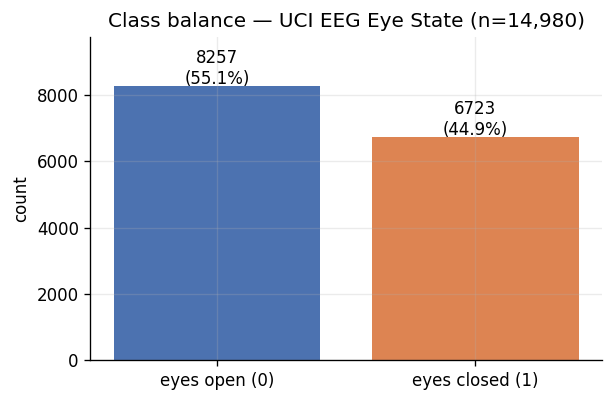
\includegraphics[width=0.5\linewidth]{01_class_balance.png}
  \caption{Class balance of the UCI~\#264 EEG eye-state dataset. The
  majority class (eyes open) sets the random-guess baseline at $0.5512$.}
  \label{fig:balance}
\end{figure}

A purely structural feature of this dataset is the heart of the study. The
labels change rarely: the recording contains only \textbf{24 contiguous
label runs} (the subject opens or closes their eyes only $23$ times in
$\sim$117\,s), with run lengths ranging from under a hundred to several
thousand consecutive samples (Figure~\ref{fig:timeseries}). Consequently
the lag-1 autocorrelation of any single voltage channel is
$\approx 0.997$---adjacent samples are nearly identical---and the label,
being piecewise-constant over long runs, has very high short-lag
autocorrelation: $\approx 1.0$ at lag~1, $\approx 0.83$ at lag~50
($\approx 0.4$\,s), crossing zero only at very long lags
(Figure~\ref{fig:autocorr}).

\begin{figure}[t]
  \centering
  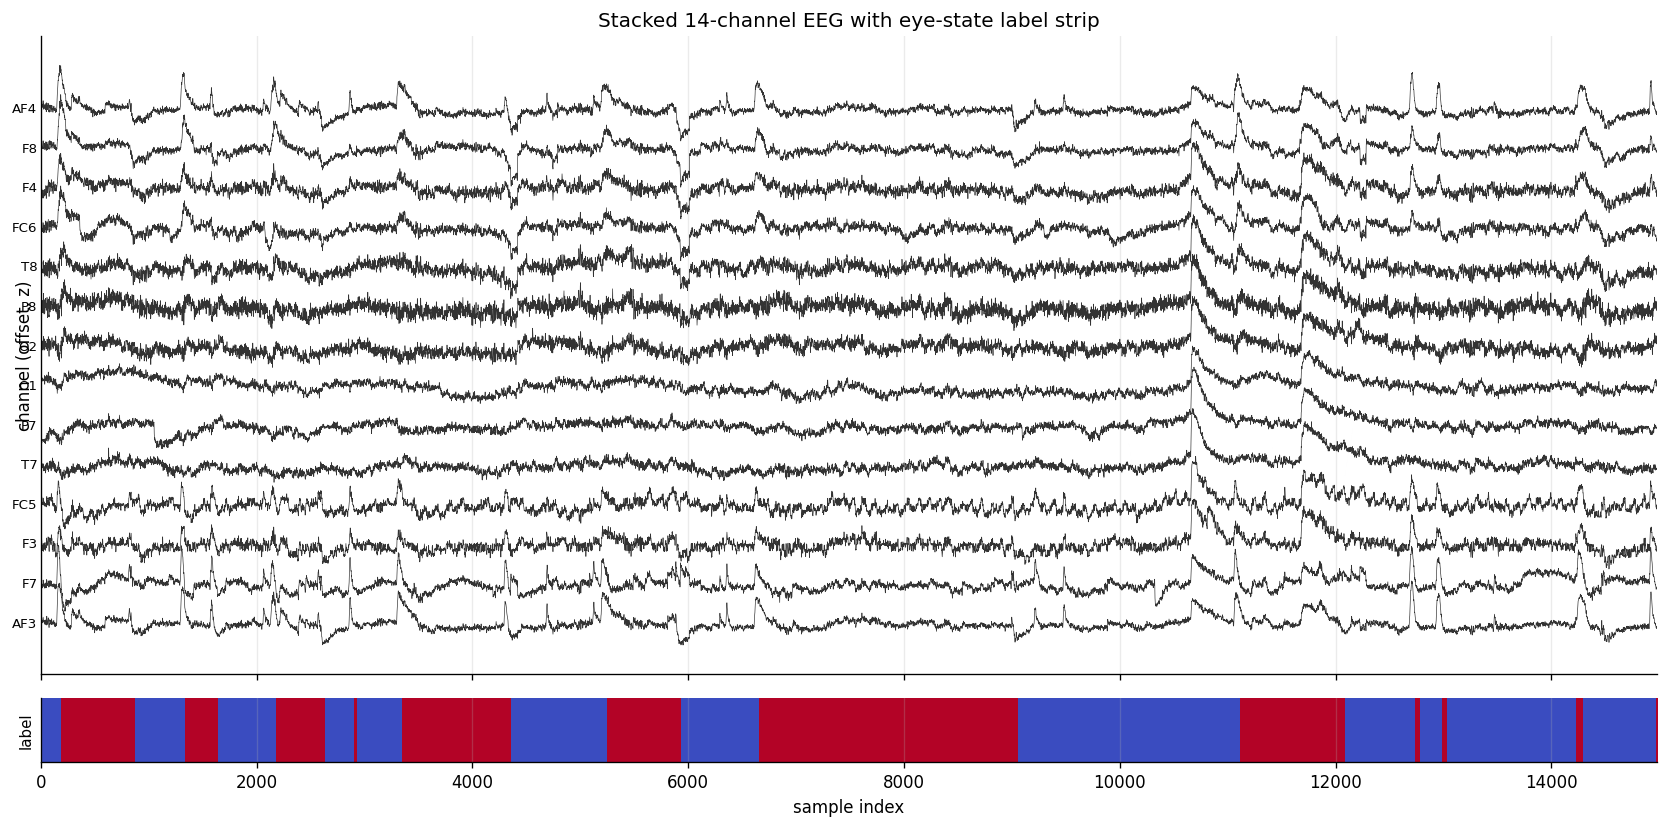
\includegraphics[width=0.66\linewidth]{04_timeseries_with_label.png}
  \caption{Raw 14-channel EEG voltages (top) with the eye-state label strip
  (bottom). Channels are continuous and smooth on the millisecond scale; the
  label is piecewise-constant over multi-second runs.}
  \label{fig:timeseries}
\end{figure}

\begin{figure}[t]
  \centering
  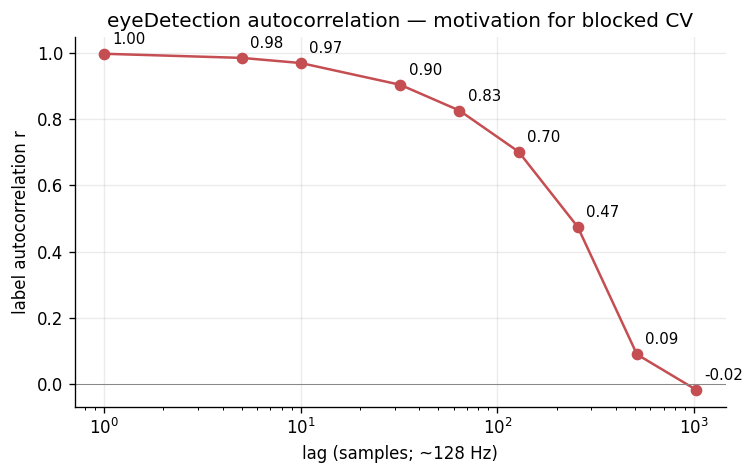
\includegraphics[width=0.56\linewidth]{08_label_autocorrelation.png}
  \caption{Autocorrelation of the binary \texttt{eyeDetection} label across
  lags $1$--$1000$. The label is essentially identical to itself for the
  first $\sim$100 samples ($\sim$0.8\,s) and only decorrelates at very long
  lags. This is the structural reason shuffled CV leaks: a sample's nearest
  neighbour in time is almost always in its own class.}
  \label{fig:autocorr}
\end{figure}

This is the structural problem at the heart of the report: \emph{any} CV
protocol that splits samples uniformly at random leaves each test sample
with a near-duplicate in its own training set. A model whose prediction
depends on per-sample similarity---\knn{} with $k=1$ being the canonical
example---will appear spectacular, but the score reflects memorisation,
not a generalisable voltage-to-label rule.

\subsection{Hypothesis}

\begin{quote}
\textbf{Hypothesis.} A \knn{} classifier trained on raw 14-channel EEG
voltages can predict per-sample eye state above the $55.12\%$
majority-class baseline, but accuracy estimates obtained under shuffled
$k$-fold cross-validation will substantially exceed honest out-of-time
estimates because of temporal leakage between adjacent samples.
\end{quote}

\noindent The hypothesis has two parts and we test both: (i) the honest
accuracy beats the majority baseline, and (ii) the shuffled estimate is
inflated relative to a leakage-resistant estimate. A negative or ambiguous
result on either part would still be informative; we report exactly what we
find.

% ===========================================================================
\section{Methods}

\subsection{Approach: classification (prediction)}

The COGS~109 study guide enumerates several broad approaches (linear,
polynomial and spline regression, PCR, LDA, KNN, $K$-means, hierarchical
clustering, PCA). The target variable here is the binary
\texttt{eyeDetection} label, so \textbf{classification} is the natural
approach: we want a model that maps a 14-dimensional voltage vector to one
of two discrete labels. Regression approaches do not target a discrete
label without artificial thresholding, and clustering approaches ignore
the label entirely. We are focused on \textbf{prediction} (out-of-sample
accuracy of the eye-state label), not on inference about which channel
``causes'' an eye state; the methodological question is specifically about
how honestly we can \emph{estimate} that predictive accuracy.

\subsection{Model: $k$-nearest neighbours}

Within classification we chose \knn{} as our model. \knn{} assigns a test
sample the majority label among its $k$ nearest training samples under
Euclidean distance in the $z$-scored 14-D channel space. We chose it for
three reasons. First, it is the simplest non-parametric classifier in the
palette: it makes no distributional assumption and has exactly one
hyperparameter ($k$) controlling the bias--variance trade-off, making it
ideal for a clean single-axis hyperparameter sweep. Second---and most
importantly for this study---because \knn{} predicts from per-sample
similarity to the training set, it is the model in the palette that
\emph{most directly} exploits the lag-1 autocorrelation of EEG data; if we
want to study how CV scheme choice changes a result, picking the model
most sensitive to that choice gives the cleanest empirical signal. Third,
\knn{} at small $k$ reproduces the $\sim$97\% literature numbers on this
dataset under shuffled CV, so the leakage gap we measure is a like-for-like
comparison between an honest and a leaky estimate of the same baseline.

\subsection{Preprocessing}

\begin{enumerate}[leftmargin=1.5em,itemsep=2pt,topsep=2pt]
  \item \textbf{Outlier removal.} We drop the four samples with at least
    one channel exceeding $4$ standard deviations above the channel mean
    ($z > 4$). This is standard EEG hygiene for headset disconnections and
    artefacts; an ablation (\texttt{tables/02\_outlier\_ablation.csv}) shows
    it does not materially change downstream accuracy but stabilises
    per-channel summary statistics. Cleaning leaves $14{,}976$ samples.
  \item \textbf{Chronological split.} We split the cleaned recording
    chronologically into $80\%$ train ($n = 11{,}917$) and $20\%$ test
    ($n = 2{,}995$), inserting a \textbf{64-sample seam gap} ($0.5$\,s at
    128\,Hz) between train and test so no train sample is within half a
    second of a test sample. This is the minimum cross-partition isolation
    warranted by the autocorrelation profile in
    Figure~\ref{fig:autocorr}.
  \item \textbf{$z$-scoring (train statistics only).} We $z$-score each
    channel using the \emph{training} mean and standard deviation only,
    and reuse those parameters for the test set. $z$-scoring before the
    split would itself leak (the test set would shape the channel scale),
    so we defer it to after the split.
\end{enumerate}

\subsection{Model-selection procedure: the $k$-sweep}

The hyperparameter to tune for \knn{} is $k$, the number of neighbours that
vote. We sweep
\[
  k \in \{1,3,5,7,11,15,21,31,51,75,99,151,201\},
\]
a log-spaced, odd-only grid (odd avoids ties on a binary label) that starts
at $k=1$ (the most leakage-prone setting) and extends to $k=201$ (a local
average that should damp out lag-1 similarity if a real classification
signal exists). For each $k$ and each CV scheme we run 5-fold
cross-validation on the $z$-scored training partition and aggregate
per-fold accuracy as mean $\pm$ standard deviation. The \textbf{selected
$k$} under a scheme is the argmax of mean CV accuracy. Crucially, the
selection \emph{rule} (argmax accuracy) is identical across schemes---only
the fold-assignment rule changes.

\subsection{Cross-validation schemes (how the splitting actually works)}

We implement all three schemes ourselves rather than delegating to a
library, so we can state exactly how each one partitions the
$N = 11{,}917$ training samples into 5 folds. In every scheme each sample
appears in exactly one test fold, and a fold's training set is the
complement of its test set.

\paragraph{Scheme A --- shuffled 5-fold (leaky baseline).}
We generate an index array $[0,1,\dots,N-1]$ and apply a single
seed-fixed Fisher--Yates permutation (NumPy \texttt{default\_rng(42)}).
The shuffled indices are cut into 5 contiguous equal blocks (the last
block absorbs the remainder); block $i$ is the test set of fold $i$ and the
other four blocks are its training set. Because the permutation is uniform,
each test fold is a random $20\%$ subset spread across the whole
recording---so the immediate temporal neighbours of almost every test
sample land in the training folds. This is the standard
``\texttt{KFold(shuffle=True)}'' protocol, and the leakiest possible scheme
on a continuous time series.

\paragraph{Scheme B --- naive blocked 5-fold.}
We take the time-ordered index array \emph{without} shuffling and cut it
into 5 contiguous chunks. Fold $i$'s test set is chunk $i$ (a single
contiguous span of time); its training set is the remaining time. This
eliminates lag-$\le 1$ leakage but introduces a new problem: because the
label runs are long and unevenly distributed, individual chunks can be
near class-pure (e.g.\ one chunk at $\sim$20\% class-0 vs.\ the overall
$\sim$54\%). Per-fold accuracy variance therefore explodes and the mean can
fall \emph{below} the majority baseline. We include it to make the failure
mode visible---it is \emph{not} a scheme we recommend.

\paragraph{Scheme C --- stratified blocked 5-fold (honest).}
This is the protocol we recommend. We cut the time-ordered training
partition into $M = 100$ short contiguous segments of $\sim$119 samples
($\sim$0.93\,s) each, preserving within-segment temporal continuity. We
label each segment by its class-1 proportion, sort the segments by that
proportion, and walk the sorted list in chunks of $5$; within each chunk
the five segments are assigned to the five folds by a seed-fixed random
permutation. The effect is that each fold receives one segment from each
quintile of the class-1-proportion distribution, so every fold's class
balance is within $\sim$3\pp{} of the overall $\sim$54\% class-0 balance.
This keeps the temporal-isolation guarantee of blocked CV (neighbours stay
together inside a segment) \emph{and} restores the class-balance guarantee
of stratified CV. Figure~\ref{fig:folds} visualises the per-fold sample
assignments under all three schemes.

\begin{figure}[t]
  \centering
  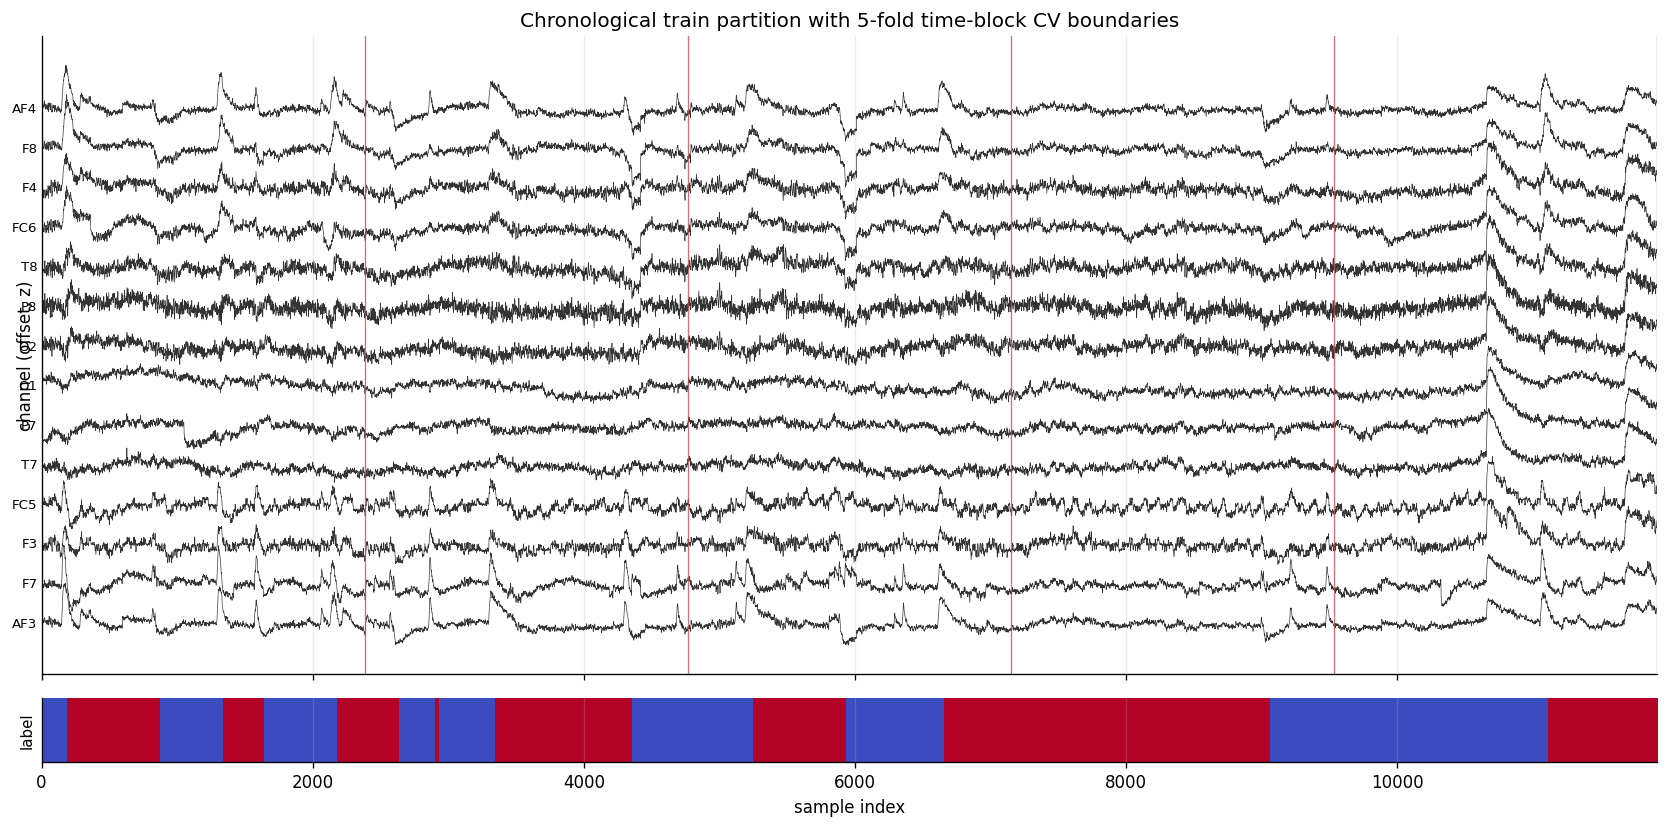
\includegraphics[width=0.7\linewidth]{04b_timeseries_with_folds.png}
  \caption{Per-fold sample assignments under the three CV schemes.
  Shuffled (top) scatters each fold across the whole recording, so temporal
  neighbours of a test sample are in the training folds. Naive blocked
  (middle) uses 5 long contiguous chunks with very uneven class balance.
  Stratified blocked (bottom) uses 100 short contiguous segments
  redistributed so each fold is class-balanced while neighbours stay
  together.}
  \label{fig:folds}
\end{figure}

\subsection{Comparison models (sanity checks)}

To test whether the leakage gap is \knn{}-specific or a generic property of
this dataset, we run the same model-selection idea on three other
classifiers from the palette. \textbf{LDA} has no tunable
hyperparameter---one accuracy per scheme. \textbf{PCA$\to$LDA} sweeps
$n_{\text{comp}} \in \{1,2,3,5,7,10\}$ and selects the $n$ maximising mean
stratified-blocked CV accuracy. \textbf{PCR-as-classifier} (ordinary least
squares on the first $n$ principal components, thresholded at $0.5$) sweeps
the same grid. These are supporting evidence, not the primary result.

\subsection{Metrics}

We report \textbf{accuracy} $= (\mathrm{TP}+\mathrm{TN})/N$ as the headline
metric for both CV and holdout, and \textbf{sensitivity} (recall for
closed$=1$) and \textbf{specificity} (recall for open$=0$) in the holdout
confusion matrices. The chronological holdout is heavily class-imbalanced
($\sim$91\% class-0, because the final segment of the recording is a long
eyes-open run), so we treat the per-fold CV numbers, not the holdout
accuracy, as the meaningful summary.

% ===========================================================================
\section{Results}

\subsection{Model selection: \knn{} under three CV schemes}

Figure~\ref{fig:ksweep} is the headline figure. It plots \knn{} mean
accuracy $\pm$ standard deviation as a function of $k$ (log scale) under all
three CV schemes on the same axes.

\begin{figure}[t]
  \centering
  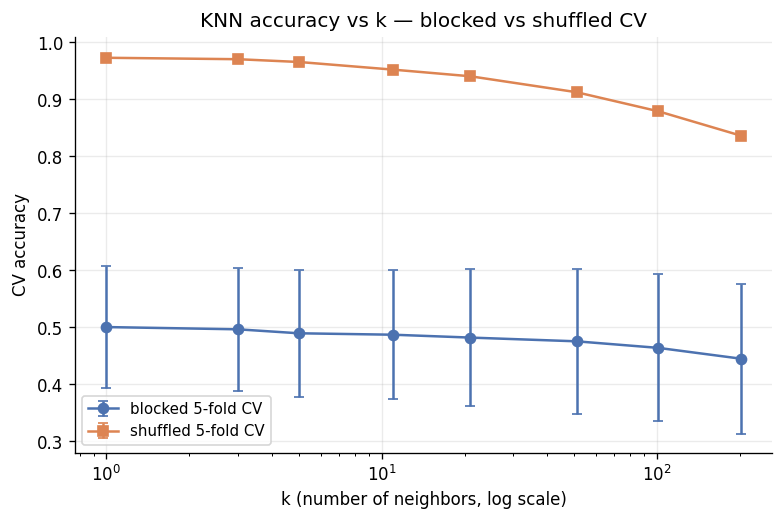
\includegraphics[width=0.7\linewidth]{11_knn_k_sweep.png}
  \caption{\knn{} model selection under three CV schemes (5-fold each; error
  bars are $\pm 1$\,SD across folds). Orange squares: shuffled CV (leaky
  baseline). Blue circles: naive blocked CV. Green diamonds: stratified
  blocked CV (honest). The horizontal dashed line is the majority-class
  baseline ($0.5512$). The open marker on each curve highlights the
  argmax-accuracy $k$ and the corresponding accuracy.}
  \label{fig:ksweep}
\end{figure}

Three observations are immediate. The shuffled curve sits near $0.97$
across all $k$, decaying roughly linearly on the log axis from $0.973$ at
$k=1$ to $\sim$0.84 at $k=201$---``nearly perfect'' everywhere. The naive
blocked curve sits near $0.50$ across all $k$, at or below the majority
baseline, with very large per-fold standard deviation ($\sim$10--13\pp);
this is fold construction failing, not the model failing
(\S\ref{sec:naive}). The stratified blocked curve peaks at $0.778$ at
$k=1$ and decays gracefully to $\sim$0.71 by $k=201$, with a much smaller
standard deviation ($\sim$2.7--4.0\pp).

Applying the argmax-accuracy rule to each scheme yields Table~\ref{tab:pick}.

\begin{table}[t]
  \centering
  \caption{Per-scheme selected $k$ and accuracy from the \knn{} $k$-sweep.
  All three schemes select $k=1$; the reported accuracies span
  $47$ percentage points.}
  \label{tab:pick}
  \begin{tabular}{lcc}
    \toprule
    CV scheme & Selected $k$ & Mean accuracy $\pm$ SD \\
    \midrule
    Shuffled (leaky baseline)        & 1 & $0.9728 \pm 0.0037$ ($\approx 97.3\%$) \\
    Naive blocked                    & 1 & $0.5004 \pm 0.1068$ ($\approx 50.0\%$) \\
    \textbf{Stratified blocked (honest)} & \textbf{1} & $\mathbf{0.7778 \pm 0.0274}$ \textbf{($\approx 77.8\%$)} \\
    \bottomrule
  \end{tabular}
\end{table}

The remarkable result is that \textbf{all three schemes select the same
hyperparameter} ($k=1$): the model-selection procedure is robust, but the
\emph{answer} it reports is not. The selected accuracy ranges from $50.0\%$
(naive blocked) to $97.3\%$ (shuffled)---a $47\pp$ spread---despite the
procedure, the model, the data, and the selected $k$ being identical.

\subsection{Complexity, flexibility, and overfitting}

For \knn{}, model flexibility is inversely related to $k$: $k=1$ is the most
flexible (a jagged, high-variance decision boundary that can fit any
training point), and large $k$ is more rigid (a smooth, high-bias boundary).
The shape of the curves in Figure~\ref{fig:ksweep} is itself diagnostic of
overfitting-via-leakage. Under \emph{honest} stratified blocked CV, accuracy
\emph{decreases} monotonically as $k$ grows from $1$ to $201$
($0.778 \to 0.710$): the flexible model genuinely generalises best, with no
sign of the usual ``too-flexible'' overfitting dip, because the signal it
exploits (short-range temporal smoothness within a segment) is real and
local. Under \emph{shuffled} CV the curve is pathologically flat-and-high
($\sim$0.97 everywhere): the model is memorising the temporal twin of each
test sample regardless of $k$. That flat-near-1 curve is the fingerprint of
leakage-driven overfitting---the estimator looks like it cannot overfit
because the ``test'' samples are duplicates of training samples. The honest
curve is the one that behaves like a real bias--variance trade-off.

\subsection{Leakage-gap analysis}

The methodological centrepiece is the \textbf{leakage gap}: the difference
between an estimator's leaky shuffled-CV accuracy and its honest
stratified-blocked-CV accuracy at the same selected hyperparameter. For
\knn{} at $k=1$,
\[
  \text{leakage gap} = 0.9728 - 0.7778 = 0.1950 \quad (\approx 19.5\pp).
\]
We attribute this gap to leakage of adjacent samples across the train/test
fold boundary, not to model quality: the model is $1$-NN in both cases and
the training partition is identical---only the fold-assignment rule changes.
Under shuffled CV the temporal neighbour of every test sample lands in a
training fold with $\sim$80\% probability and carries the same label with
$\sim$99.7\% probability; under stratified blocked CV that neighbour is
reserved into the same segment as the test sample. The honest accuracy at
$k=1$, $77.8\% \pm 2.7\%$, is nonetheless $\sim$23\pp{} above the
$55.12\%$ baseline---the classifier is far from useless, just far less
impressive than the shuffled number implies. \textbf{Both parts of our
hypothesis are therefore supported.}

\subsection{Supporting evidence: alternative classifiers}

To rule out a generic explanation, we ran the same idea on three other
classifiers (Table~\ref{tab:gaps}, Figure~\ref{fig:threeway}).

\begin{table}[t]
  \centering
  \caption{Per-model leakage gaps (shuffled CV minus stratified-blocked CV)
  at the selected hyperparameter. \knn{}'s gap is the outlier:
  $\sim$4--8$\times$ larger than any other classifier in the palette.}
  \label{tab:gaps}
  \setlength{\tabcolsep}{4pt}
  \small
  \begin{tabular}{lcccc}
    \toprule
    Model & Selected hyperparam. & Shuffled CV & Strat.\ blocked CV & Leakage gap \\
    \midrule
    LDA            & --- (no sweep) & $0.6471 \pm 0.0063$ & $0.5911 \pm 0.0474$ & $+5.6\pp$ \\
    PCA$\to$LDA    & $n=3$          & $0.5574 \pm 0.0147$ & $0.5339 \pm 0.0438$ & $+2.4\pp$ \\
    PCR (classifier)& $n=2$         & $0.5528 \pm 0.0087$ & $0.5250 \pm 0.0176$ & $+2.8\pp$ \\
    \textbf{\knn{}} & $\mathbf{k=1}$ & $\mathbf{0.9728 \pm 0.0037}$ & $\mathbf{0.7778 \pm 0.0274}$ & $\mathbf{+19.5\pp}$ \\
    \bottomrule
  \end{tabular}
\end{table}

\begin{figure}[t]
  \centering
  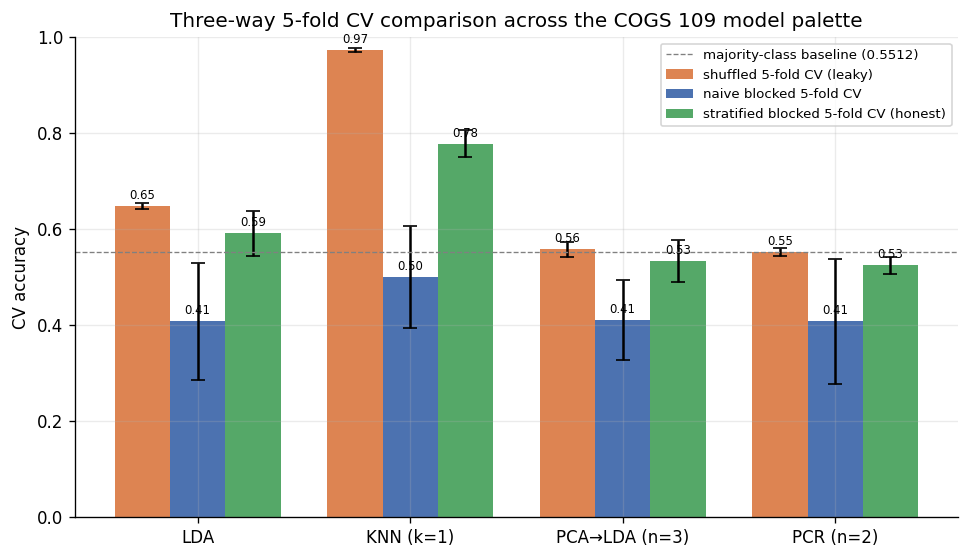
\includegraphics[width=0.66\linewidth]{14_cv_comparison_three_way.png}
  \caption{Three-way 5-fold CV accuracy across the four palette
  classifiers. Orange: shuffled; blue: naive blocked; green: stratified
  blocked. The \knn{} bar group has by far the largest
  shuffled-to-stratified-blocked gap, consistent with \knn{} being uniquely
  vulnerable to lag-1 autocorrelation.}
  \label{fig:threeway}
\end{figure}

The pattern is exactly what we expect if the gap is caused by per-sample
autocorrelation. LDA's decision rule is a single global linear projection
of the 14-D space onto a 1-D axis; it cannot exploit per-sample similarity,
so its gap is small ($5.6\pp$). PCA$\to$LDA and PCR both project to a
low-dimensional subspace before deciding, destroying most of the
high-frequency sample-to-sample similarity \knn{} relies on; their gaps are
smaller still ($2.4$ and $2.8\pp$). \knn{} at $k=1$ is the only classifier
whose prediction depends on the identity of the single nearest training
sample---and its gap is $4$--$8\times$ larger than any other.

\subsection{Model estimation: final parameters and accuracy}

\paragraph{Final model and ``parameters''.}
The selected model is \knn{} with $k=1$ on the $z$-scored 14-channel
features. \knn{} is non-parametric, so the ``fitted parameters'' are not
coefficients but (i) the selected hyperparameter $k=1$ and (ii) the stored
training set itself together with the per-channel $z$-scoring constants
$(\mu_c,\sigma_c)$ estimated on the full training partition (persisted in
\texttt{data/processed/scaler.json}). For a concrete parametric contrast,
the LDA comparison model \emph{does} have estimable coefficients: its
14-channel discriminant weights (estimated on the full training set) are
reported in \texttt{figures/10\_lda\_coefficients.png}, with the
occipital/parietal channels (O1, O2, P7, P8) carrying the largest
magnitude---consistent with eye-closure altering posterior alpha rhythms.

\paragraph{Final accuracy.}
The honest cross-validated estimate of the selected model
($k=1$, stratified blocked CV) is $\mathbf{77.8\% \pm 2.7\%}$, versus the
$55.12\%$ majority baseline. As a confirmatory out-of-sample check,
Figure~\ref{fig:confusion} shows per-model confusion matrices on the $20\%$
chronological holdout. The holdout is $\sim$91\% class-0, so its accuracy is
dominated by specificity and we do not over-interpret it; we did not
rebalance it because doing so would itself introduce leakage. The CV
numbers above are the headline estimate.

\begin{figure}[t]
  \centering
  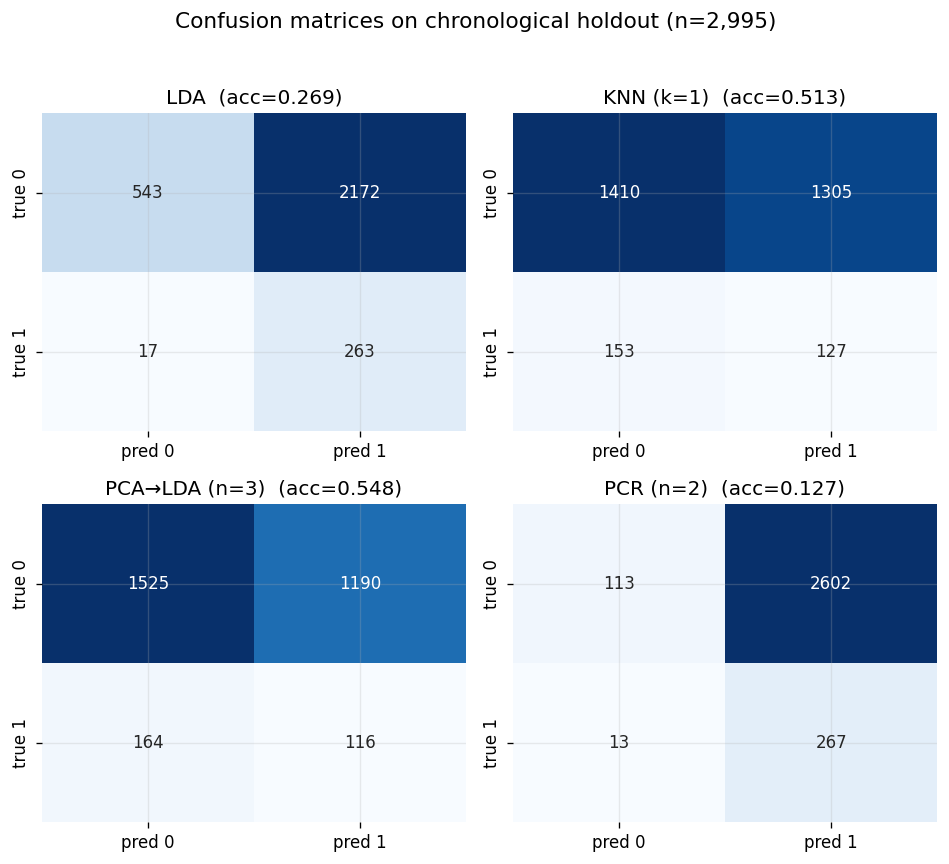
\includegraphics[width=0.64\linewidth]{15_confusion_matrices.png}
  \caption{Per-model confusion matrices on the $20\%$ chronological holdout
  test set (rows: true; columns: predicted). The holdout is dominated by
  eyes-open samples ($\sim$91\% class-0), so accuracy here is mostly driven
  by specificity. The number in each panel is that model's holdout accuracy.}
  \label{fig:confusion}
\end{figure}

% ===========================================================================
\section{Conclusions and Discussion}

\subsection{What we conclude about the hypothesis}

Both parts of our hypothesis hold. (i)~The honest \knn{} accuracy
($77.8\%$) beats the majority baseline ($55.12\%$) by $\sim$23\pp, so raw
14-channel voltages do carry a genuine, generalisable eye-state signal.
(ii)~The shuffled-CV estimate ($97.3\%$) is inflated by $19.5\pp$ relative
to the honest estimate, and that inflation is leakage attributable purely
to the CV scheme: the model, the selected $k$, and the training data are
identical across schemes.

\takehome{Shuffled CV says we have a 97\% classifier. Honest stratified
blocked CV says we have a 78\% classifier. The difference is leakage, not
signal.}

\subsection{Why \knn{} is uniquely vulnerable}
A $1$-NN classifier predicts the class of the single nearest training
neighbour. Because the lag-1 channel correlation is $\approx 0.997$, the
nearest neighbour in feature space is almost always the temporal neighbour.
Under shuffled CV that neighbour is in a training fold $\sim$80\% of the
time and shares the test label $\sim$99.7\% of the time, so $1$-NN trivially
exceeds $95\%$ without learning any voltage-to-state rule. Under stratified
blocked CV the temporal neighbour is reserved into the test sample's own
segment, forcing \knn{} onto the next-nearest non-adjacent sample, and
accuracy drops to $77.8\%$. Models that average over many samples (LDA,
PCA$\to$LDA, PCR) cannot exploit this and show only $2$--$6\pp$ gaps.

\subsection{Why naive blocked CV underperforms the baseline}
\label{sec:naive}
The five contiguous chunks are not class-balanced: with only $23$ label
transitions in the recording, several chunks straddle few or zero
transitions, and per-chunk class proportions stray far from the global
$55/45$ split. A classifier trained on four mostly-open chunks then
predicts ``open'' on a held-out mostly-closed chunk, scoring \emph{below}
the majority baseline. This is a fold-stratification failure, not a model
failure; stratifying contiguous segments (Scheme C) fixes it, which is why
stratified blocked CV recovers $\sim$28\pp{} over naive blocked.

\subsection{Implications and future work}
A non-trivial fraction of tutorials and student projects on this dataset
report $95$--$98\%$ \knn{} accuracy under shuffled $k$-fold. Our analysis
suggests those numbers are a CV-protocol artefact: the honest accuracy is
$77.8\%$ and the extra $\sim$20\pp{} is adjacent-sample leakage. This echoes
broader cautions about i.i.d.\ CV on autocorrelated signals (Bergmeir \&
Ben\'itez, 2012). The practical recommendation is to use blocked,
class-stratified CV (or an explicit out-of-time holdout with a seam gap)
whenever samples are temporally autocorrelated. Limitations of our study:
it is a single subject on consumer hardware over $\sim$117\,s, and we use
per-sample voltages with no windowed features. Future work should (i)~add
windowed features (rolling means/variances, lagged values), which would
give \knn{} more meaningful neighbours and likely shrink the leakage gap;
(ii)~test cross-subject generalisation on a multi-subject corpus; and
(iii)~extend the $k$ sweep to characterise the leakage curve more finely.
The project is, above all, a worked example of how a methodologically sound
model-selection procedure can still be misled by an upstream choice---the
CV scheme---that has nothing to do with the model itself.

% ===========================================================================
\section*{References}
\begin{enumerate}[leftmargin=1.5em,itemsep=2pt,topsep=2pt]
  \item Roesler, O. (2013). \emph{EEG Eye State Data Set}. UCI Machine
    Learning Repository, id~\#264.
    \url{https://archive.ics.uci.edu/dataset/264/eeg+eye+state}
  \item Mukamel, R. (2026). \emph{COGS 109 --- Modelling and Data Analysis,
    Spring 2026 Study Guide}. UC San Diego.
  \item James, G., Witten, D., Hastie, T., \& Tibshirani, R. (2021).
    \emph{An Introduction to Statistical Learning}, 2nd ed. Springer.
  \item Bergmeir, C., \& Ben\'itez, J.~M. (2012). On the use of
    cross-validation for time series predictor evaluation.
    \emph{Information Sciences} 191:192--213.
  \item Pedregosa, F., et al. (2011). Scikit-learn: Machine learning in
    Python. \emph{Journal of Machine Learning Research} 12:2825--2830.
\end{enumerate}

\end{document}
